\subsection{LWM2M: CoAP and HTTP with Leshan}


LWM2M is the fundamental ingredient in the broker. It provides a REST API for both CoAP and HTTP which can both be modified to serve the needs of the system. Leshan operates with a server/client infrastructure. Thus the broker runs a server module and other devices connecting to it use a client module. The android app and the cloud service take advantage of the HTTP protocol and the end-device uses the CoAP protocol.

\begin{figure}[h]
	\begin{center}
		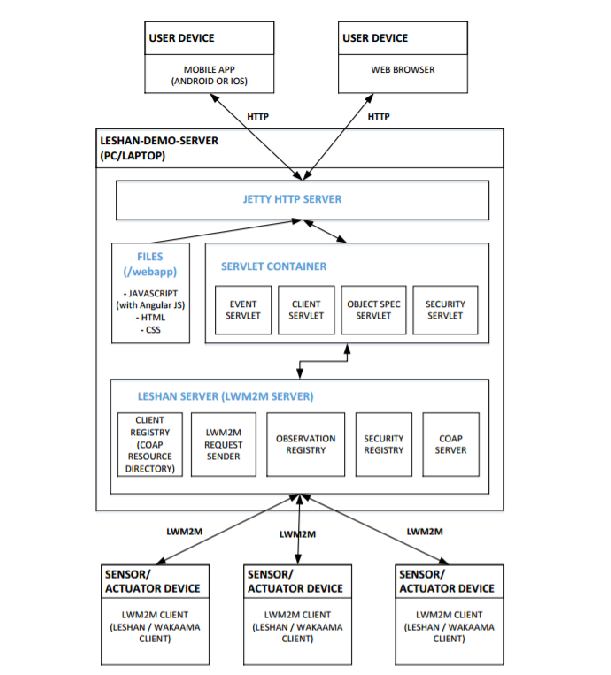
\includegraphics[width=1.3\linewidth]{img/LeshanArc}
		\caption{Architecture of Leshan Server used in implementation} 
		\label{fig:fig3}
	\end{center}
\end{figure}

Event Servlet Functions:Listening to new registrations using RegistrationListener component. Whenever a new registration happens location from database is automatically written into the client based on the order of registration.The location is also updated by the cloud service later if needed. 

Updating the database whenever a value change is detected using ObservationListener component. Observation requests for UserId(Sensor),SenosrState,BehaviourDeployment,Light State, Light Color are requested during registration. A database is created (series of text files) to record and update the Light settings for different users. Whenever a value change is detected in any of these the 'new value' function in the Observation Listener gets activated and the values are updated into database. Inside this function a routine is also made to write the appropriate light values and user information to the light device from database based on the type of behaviour deployment,SensorState and the userId(Sensor).


ClientServletFunctions$(http://serverAddress/api/clients/*)$:\\
Handles all the requests from the cloud service and responds with appropriate responses.Typical requests include reading and writing the resource values using endpointname/Objid/instnId/rsrcId path in the URL.It also handles the handles read and write requests from User App using the same protocol.


SecurityServletFunctions$(http://server_address/api/clients/*)$:\\
Handles storing information of user details in the database  when sent by cloud service and handles authentication of the user from UserApp using these details.

ObjectSpecServlet$(http://server_address/objectspecs/*)$:\\
Handles requests for getting information on objects supported and corresponding details for implementation.


ClientRegistry:Stores the information of registered Clients.

ObservationRegistry:Stores the information on Observation requests created.

LWM2M Request Sender: Responsible for sending request objects(Read,Write,Observe) to the clients.

COAP server: Server for handling COAP messages from clients.

Jetty HTTP Server:HTTP server for handling http requests from USERAPP and Cloud service.

FILES:Files for storing values of different observations(database) and files for creating and updating the Leshan Server page. 

\subsection{User app: Android} 
User App is used to update the light settings of the the user. The settings can be accessed only after logging in with the userId and password. The details are sent to the broker using HTTP protocol(GET). The broker receives the information of all the userID's and their corresponding passwords from cloud service during the "Set User Account" phase. While the intended application is to get the change the corresponding user light settings when logged in, due to a misunderstanding we implemented an which could modify the current light settings of any client active at that moment. Hence any user when logged in with correct details can modify the light settings(provided the client has  a light device) of all the clients active at that point of time.

\begin{figure}[h]
	\begin{center}
		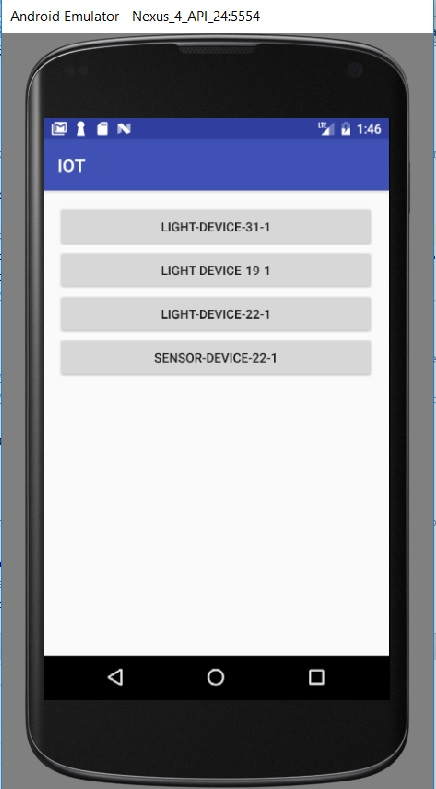
\includegraphics[width=.7\linewidth]{img/android1}
		\caption{Client Details in android App}
		\label{fig:fig3}
	\end{center}
\end{figure}


\begin{figure}[h]
	\begin{center}
		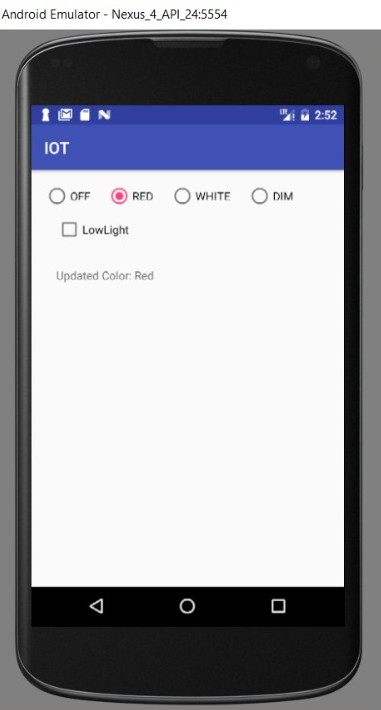
\includegraphics[width=.7\linewidth]{img/androidapp}
		\caption{Updating Light Values from User App }
		\label{fig:fig4}
	\end{center}
\end{figure}



Note:During the interactions between user app and the broker the IP address of broker is manually set during the initialization phase of the app. No service discovery is used in this case.